% Chapter 3

\chapter{Methodology} % Main chapter title

\label{Chapter3} % For referencing the chapter elsewhere, use \ref{Chapter3} 

%----------------------------------------------------------------------------------------
To quantify the environmental footprint of the financial systems in the United States and the Eurozone, this thesis adopts the macroeconomic framework developed by \textcite{jondeau_environmental_2026}. The methodology links financial exposures to environmental pressures in three steps. First, FWTW matrices are used to estimate the effective financing provided by each financial-institution group to each real-economy agent, after accounting for chains of financial intermediation. Second, these exposures are normalized by the total outstanding claims on each real-economy agent to obtain attribution factors. Third, the attribution factors are combined with environmental footprints derived from EXIOBASE to calculate the environmental pressures financed by different parts of the financial system.

While this framework allows environmental pressures to be attributed to specific categories of financial institutions, real-economy agents, and asset classes, it relies on several simplifying assumptions. Consequently, as noted by the original authors, finely disaggregated results should be interpreted with caution, while aggregate system-wide estimates are generally more robust.


This macro-based approach directly complements traditional portfolio-level methodologies. Bottom-up approaches, though useful for granular assessments, rely heavily on voluntary corporate disclosures and often provide an incomplete picture of systemic risk due to missing data from unlisted firms and undisclosed portfolios. By capturing the full chain of financial intermediation, spanning all sectors and asset classes without double counting, this top-down method bridges the empirical gaps left by selective corporate reporting.

\section{Effective financing by financial institutions to economy sectors}
\label{sec:effective_financing}

Financial institutions are treated as "intermediate industries" from an accounting perspective. For a given asset class $a$, they hold direct claims on real-economy agents, denoted by $V_{FR,t}^{(a)}$, as well as claims on other financial institutions, denoted by $V_{FF,t}^{(a)}$. However, considering direct holdings alone is not sufficient, as a financial institution $f$ may hold claims on another financial institutions $f'$ that in turn holds claims on a real-economy agent $k$. To accurately measure the effective financing provided by financial institutions to real-economy agents, it is therefore necessary to account for the entire chain of intermediation.

\textcite{jondeau_environmental_2026} aggregate FWTW matrices across all asset classes to obtain overall financial relations among all agent groups, $V_t = \sum_{a \in \mathcal{A}} V_t^{(a)}$. They then define the (row-normalized) share matrix $S_t$, with elements
\begin{equation}
S_{ij,t} = \frac{V_{ij,t}}{\sum_{j'=1}^{N} V_{ij',t}}, \quad i,j = 1,\ldots,N.
\end{equation}
representing the share of agent $i$'s holdings invested in claims issued by agent $j$. This normalization makes $S_t$ dimensionless, with entries in $[0,1]$. Since real-economy agents are treated as final issuers, the look-through procedure is applied only to claims among financial institutions, captured by the financial block $S_{FF,t}$.

To trace financing through the network of financial institutions, the direct claims of financial institutions on real-economy sectors, $V_{FR,t}$, must be adjusted for indirect exposures created by financial intermediation. For example, a financial institution may not finance a real-economy issuer directly, but may hold claims on another financial institution that does. In this case, the exposure is transmitted through the financial-institution block of the allocation matrix, $S_{FF,t}$.

Starting from direct financing of the real economy, each additional layer of intermediation adds another multiplication by $S_{FF,t}$. The effective exposure of financial institutions to real-economy sectors is therefore given by the infinite expansion
\begin{equation}
W_{F,t}
= \left(I_{n_F} + S_{FF,t} + S_{FF,t}^2 + \cdots \right)V_{FR,t}
= (I_{n_F} - S_{FF,t})^{-1}V_{FR,t},
\label{eq:effective_exposure}
\end{equation}
provided that the spectral radius of $S_{FF,t}$ satisfies $\rho(S_{FF,t}) < 1$.

The matrix $(I_{n_F} - S_{FF,t})^{-1}$ plays the role of a Leontief inverse in the financial input-output system. Analogous to the standard input-output model, where final demand generates production requirements through successive rounds of intermediate inputs, real-economy financing is transmitted here through successive rounds of financial intermediation. This look-through procedure reallocates exposures from financial counterparties to their underlying real-economy issuers, thereby capturing both direct and indirect financing links while avoiding repeated attribution of the same exposure. The resulting matrix $W_{F,t}$ $(n_F \times n_R)$, measures the effective financing provided by each financial-institution group $f$ to each real-economy sector $k$ after accounting for all intermediation layers.

\section{Environmental Impacts by Real-economy Agents}

\subsection{Multi-region Input-Output Model}

To understand the structure of the EXIOBASE database, it is useful to review the key components of the multi-regional input-output (MRIO) model. Figure~\ref{fig:MRIO} illustrates a typical MRIO data structure.

\begin{figure}[h]
    \centering
    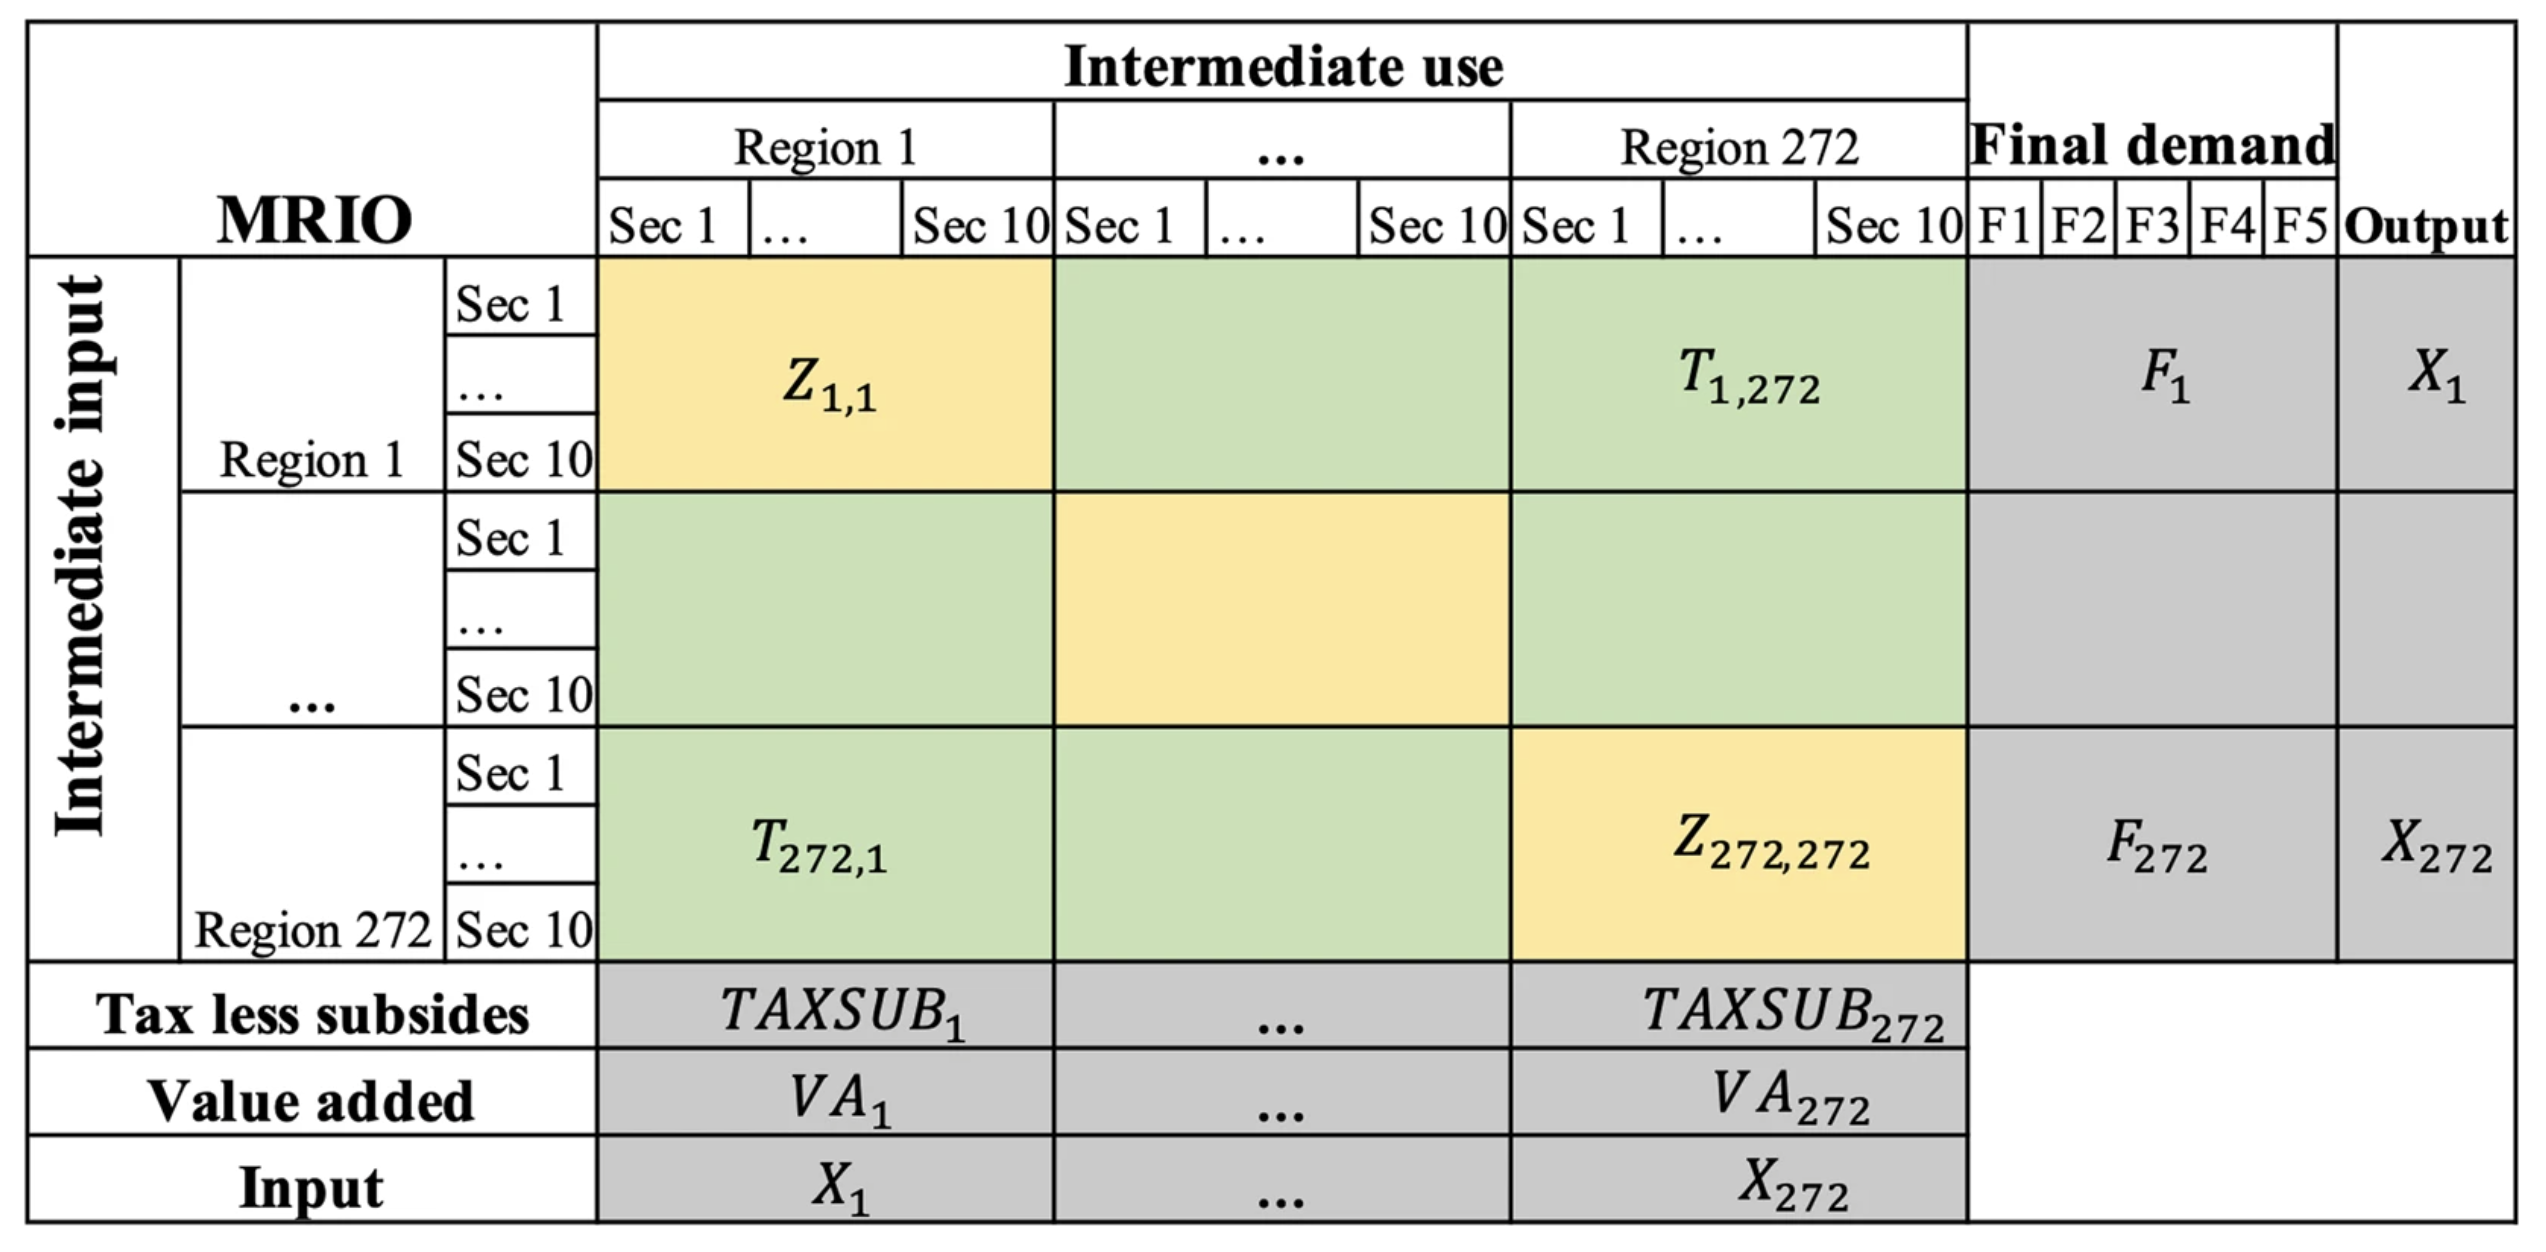
\includegraphics[width=\textwidth]{Figures/MRIO.png}
    \caption[Illustration of a MRIO table]{Illustration of a MRIO table.}
    \label{fig:MRIO}
    \vspace{0.2em}
    {\footnotesize \textit{Source: \cite{ huang_european_2023}}}
\end{figure}

Countries and sectors are indexed by $c = 1, \ldots, n_C$ and $s = 1, \ldots, n_S$, respectively. In EXIOBASE, this corresponds to $n_C = 49$ countries/regions and $n_S = 163$ sectors. Stack all country-sector pairs into a single index $i = 1, \ldots, n$ with $n = n_C n_S$. Let $e_n$ be a $(n \times 1)$ vector of ones and $I_n$ the $(n \times n)$ identity matrix. 

The EXIOBASE database provides the following key matrices and vectors:
\begin{itemize}
    \item The gross output vector $x_t \in \mathbb{R}^{n \times 1}$, where each element represents the total output of a country-sector.

    \item The inter-industry transaction matrix $Z_t \in \mathbb{R}^{n \times n}$, where each element $Z_{ij,t}$ denotes the monetary flow from sector $i$ to sector $j$. Rows correspond to supplying sectors, while columns correspond to using sectors.

    \item The final demand matrix $Y_t \in \mathbb{R}^{n \times n_C n_Y}$, where $n_Y = 7$ denotes the seven categories of final demand: household consumption, consumption by non-profit institutions serving households (NPISH), government consumption, gross fixed capital formation, changes in inventories, changes in valuables, and exports. Each column corresponds to a country-category pair.

    \item The matrix of technical coefficients $A_t \in \mathbb{R}^{n \times n}$, defined as $A_t = Z_t \,\mathrm{diag}(x_t)^{-1}$, where each element $A_{ij,t} = Z_{ij,t} / x_{j,t}$ represents the input from sector $i$ required to produce one unit of output in sector $j$.
\end{itemize}

Let $h^{(c)} \subset \{1, \ldots, n_C n_Y\}$ denote the set of final-demand columns of country $c$ and let $D_H(\mathcal{H})$ be the $(n_C n_Y \times n_C n_Y)$ diagonal selector with ones on indices in $\mathcal{H}$. With these notations, the final demand in country $c$, denoted by $y_t^{(c)}$, is the sum of the $n_Y$ groups for the country, $y_t^{(c)} = Y_t\, D_H\!\left(h^{(c)}\right) e_{n_C n_Y}$. We collect the final demand for all countries and define the total final-demand $(n \times 1)$ vector $y_t = \left(y_t^{(1)}, \ldots, y_t^{(n_C)}\right)e_{n_C}$. These quantities are measured in monetary units.

Total output can be expressed as the sum of intermediate and final demand:
\begin{equation}
x_t = A_t x_t + y_t = (I_n - A_t)^{-1} y_t = \mathcal{L}_t y_t,
\end{equation}
where $\mathcal{L}_t$ denotes the Leontief inverse matrix. 
This equation constitutes the core of the input-output model, linking total production to final demand through direct and indirect independences between economic sectors.

\subsection{Environmental Extensions}
\label{sec:environmental extensions}

We now introduce environmental pressures. For each indicator, EXIOBASE provides 
(i) direct production pressures by industry, measured by the $(1 \times n)$ vector $F_t$, and 
(ii) direct final-use pressures that cannot be attributed to production activities (e.g., fuel combustion in private transport), measured by the $(1 \times n_C n_Y)$ vector $F_{Y,t}$. 

The pressure intensity per unit of output is $S_t = F_t \, \mathrm{diag}(x_t)^{-1}$, and the pressure intensity per unit of final demand is $M_t = S_t\mathcal{L}_t $ (also referred to as the total supply-chain multipliers). The production-related footprint associated with final demand $y_t^{(c)}$ is $M_ty_t^{(c)}$.

The set of industries in country $c$ is denoted by $\mathcal{I}^{(c)} \subset \{1, \ldots, n\}$. Let $D(S)$ denotes the $(n \times n)$ diagonal selector matrix with ones on indices in $S$ and $D_H(\mathcal{H})$ denotes the $(n_C n_Y \times n_C n_Y)$ diagonal selector with ones on indices in $\mathcal{H}$.

While this framework accommodates any EXIOBASE environmental indicator, this thesis primarily focuses on financed emissions. To maintain consistency with the climate-finance literature, the mathematical exposition uses GHG terminology, specifically, emissions ($E$), financed emissions ($FE$) and carbon intensity ($CI$). However, the identical calculations apply to other environmental footprints by substituting the target metric.

In production-based (or territorial) accounting (PBA), the footprint of country $c$ is the sum of direct domestic production pressures and direct domestic final-use pressures:
\begin{equation}
E^{(c)}_{\text{PBA},t} = F_t \, D(\mathcal{I}^{(c)}) \, e_n + F_{Y,t} \, D_H(h^{(c)}) \, e_{n_C n_Y}
\end{equation}

In consumption-based accounting (CBA), the footprint of country $c$ allocates the full supply-chain pressures to domestic final demand, regardless of where pressures occur:
\begin{equation}
E^{(c)}_{\text{CBA},t} = M_t Y_t \, D_H(h^{(c)}) \, e_{n_C n_Y} + F_{Y,t} \, D_H(h^{(c)}) \, e_{n_C n_Y}
\end{equation}

Finally, environmental pressures are attributed to mutually exclusive agent groups. To map industries to real-economy agents, \textit{Private households with employed persons} are assigned to households (HH), \textit{Public administration and defense and compulsory social security} to government (GG), and \textit{Financial intermediation and auxiliary to financial intermediation} to financial institutions (FI). All remaining industries are classified as non-financial corporations (NFC).  

For the mapping from final demand to agents, let $h(k) \subseteq \{1, \ldots, n_C n_Y\}$ denote the set of final-demand columns associated with agent group $k$. Final consumption by households and NPISH is assigned to HH, while government expenditure is assigned to GG. The remaining columns are attributed to NFC; however, final-use pressures for NFC are zero for the indicators considered, as NFC sectors are typically not final users in the economy.

For a given country $c$, environmental footprint attributed to agent group $k$ are defined as
\begin{equation}
E_{k,t}^{(c)} = F_t \, D(\mathcal{I}^{(c)} \cap \mathcal{I}_k)\, e_n 
+ F_{Y,t} \, D_H(h^{(c)} \cap h(k))\, e_{n_C n_Y}
\label{eq:emissions}
\end{equation}

For the rest of the world, I group individual countries into broader regional aggregates, such as North America, Europe, Japan-Pacific, and emerging economies. Environmental footprints are first calculated at the country level. Specifically, for each country $c$ belonging to a given region, I compute $E_{k,t}^{(c)}$ using Equation \ref{eq:emissions}. I then sum these country-level values across all countries in the region to obtain regional totals by real-economy agent group.

Although total foreign claims can be decomposed by region, the effective-exposure matrix obtained from the financial input-output framework identifies foreign issuers only as one aggregate RoW category. Therefore, the regional environmental profiles cannot be directly assigned to separate regional effective exposures. Instead, they are used to construct alternative environmental factors for the aggregate RoW issuer group. This allows the analysis to examine how the estimated environmental footprint of foreign exposures changes under different assumptions about the regional composition of RoW.

\section{Environmental Footprints of Financial Systems}
\label{sec:3.3}

To attribute the environmental pressures generated by real-economy agents to their financiers, I follow the proportional attribution logic used in financed-emissions accounting. Under this approach, environmental pressures are allocated to financial institutions according to their share of financing in the issuer's total financing base, regardless of the specific financial instrument through which the exposure is held. I therefore aggregate all classes of claims, including equity, debt securities, loans, and other financial instruments, into a common attribution base, denoted by $TC_{k,t}$, which represents total claims on real-economy agent group $k$.

For households, however, I follow \textcite{jondeau_environmental_2026} and use total assets rather than total claims, while retaining the notation $TC_{\mathrm{HH},t}$. This adjustment reflects the fact that household environmental pressures arise largely from consumption and asset ownership rather than from debt-financed production activities. Normalizing by total assets therefore provides a more appropriate measure of the economic resources controlled by households and their associated environmental footprint.

The effective, or look-through, exposure of financial-institution category $f$ to real-economy agent group $k$ at time $t$, denoted by $W_{f,k,t}$, is obtained from the matrix $W_{F,t}$ defined in Equation \ref{eq:effective_exposure}. Since funds raised through different financial instruments are treated as part of a common financing base, the attribution factor of institution category $f$ with respect to agent group $k$ is defined as
\begin{equation}
AF_{f,k,t} = \frac{W_{f,k,t}}{TC_{k,t}}.
\end{equation}
The environmental pressure financed by institution category $f$ through its exposure to group $k$ is then given by
\begin{equation}
FE_{f,k,t} = AF_{f,k,t} E_{k,t}
= \frac{W_{f,k,t}}{TC_{k,t}} E_{k,t},
\end{equation}
where $E_{k,t}$ denotes the GHG emissions or other environmental footprint of real-economy agent group $k$. For domestic issuers, $E_{k,t} \equiv E_{k,t}^{(\mathrm{home})}$, as defined in Equation \ref{eq:emissions}. For foreign issuers, $E_{k,t}$ is constructed from the regional environmental profiles described in Section \ref{sec:environmental extensions}. The corresponding attribution base, $TC_{k,t}$, is defined over the same regional coverage, ensuring that environmental footprints and financial claims are measured consistently.

Let $W_{f,t}$ denote the total effective exposure of financial-institution category $f$:
\begin{equation}
W_{f,t} = \sum_{k=1}^{n_R} W_{f,k,t}.
\end{equation}
The total financed environmental footprint of category $f$ is then
\begin{equation}
FE_{f,t}
= \sum_{k=1}^{n_R} \frac{W_{f,k,t}}{TC_{k,t}} E_{k,t}
= W_{f,t} \sum_{k=1}^{n_R}
\underbrace{\frac{W_{f,k,t}}{W_{f,t}}}_{w_{f,k,t}}
\times
\underbrace{\frac{E_{k,t}}{TC_{k,t}}}_{CI_{k,t}}.
\label{eq:financed_emis_fi}
\end{equation}
Equation \ref{eq:financed_emis_fi} shows that the financed environmental footprint of institution category $f$ can be decomposed into two components: the total size of its effective exposure, $W_{f,t}$, and the weighted average environmental intensity of the real-economy agents to which it is exposed. The portfolio weight $w_{f,k,t}$ measures the share of group $k$ in category $f$'s effective exposure, while $CI_{k,t}$ denotes the environmental intensity of group $k$.

At the level of the aggregate financial system, let $W_{k,t}$ denote total effective financing received by real-economy group $k$:
\begin{equation}
W_{k,t} = \sum_{f=1}^{n_F} W_{f,k,t}.
\end{equation}
The total effective exposure of the financial system is
\begin{equation}
W_t = \sum_{k=1}^{n_R} W_{k,t}
= \sum_{f=1}^{n_F} W_{f,t}.
\end{equation}
Aggregating across all financial-institution categories gives
\begin{equation}
FE_t
= \sum_{f=1}^{n_F} \sum_{k=1}^{n_R}
W_{f,t}
\underbrace{\frac{W_{f,k,t}}{W_{f,t}}}_{w_{f,k,t}}
\underbrace{\frac{E_{k,t}}{TC_{k,t}}}_{CI_{k,t}}
= W_t \sum_{k=1}^{n_R} \frac{W_{k,t}}{W_t} CI_{k,t}.
\end{equation}
Thus, the financed environmental footprint of the macro-financial system is the product of total effective financial exposure, $W_t$, and the system-wide weighted average environmental intensity of the real economy.

Although \textcite{jondeau_environmental_2026} discuss the assumptions and robustness of this framework in detail, its key premise is that aggregate financial exposures can be allocated proportionally to the outstanding financing base of each real-economy agent group. The resulting measure should therefore be interpreted as a macro-level attribution of environmental pressures through the structure of financial intermediation. It captures how the financial system as a whole is connected to environmentally intensive activities, rather than the institution-specific portfolio choices that would be observed in micro-level holdings data.